\section{Compressed Sensing Image Reconstruction for MeerKAT} \label{intro}
Image reconstruction problems arise in a variety of fields. Noise from different sources like external interference, loss of samples, or the instrument itself, all introduce corruptions that a reconstruction algorithm should remove. In a sense, we need a model for what the truly observed image can look like and filter out the structures due to noise. A reconstruction algorithm needs a prior for what the image is. 

This has led to the theory of Compressed Sensing\cite{candes2006robust, donoho2006compressed}, which allows us to model the reconstruction as a convex optimization problem. It gives us a theoretical framework for the analysis of reconstruction algorithms. Compressed Sensing gives us theoretical guarantees that, under the right prior, the algorithm is virtually guaranteed to reconstruct the observed image, potentially above the accuracy limit of the instrument.

In this work we apply the theory of Compressed Sensing to the reconstruction problem of Radio Interferometers. More specifically, we apply it on the MeerKAT interferometer, which poses the problem on a new scale of data volume. New Interferometers measure billions of Fourier components, which get reconstructed to a single image. The raw measurements easily take up hundreds of gigabytes of space. The current state of the art reconstruction is based on the CLEAN\cite{rich2008multi, rau2011multi} algorithm. Although newer Compressed Sensing reconstructions showed superior image quality\cite{girard2015sparse, dabbech2018cygnus}, they have higher runtime costs than CLEAN.

CLEAN and current Compressed Sensing algorithms use the non-uniform FFT approximation to cycle between measurements and image space. Compressed Sensing algorithms need more cycles to converge to an image, which is one source of the higher runtime costs. In this project we investigate alternatives to the non-uniform FFT for Radio Interferometers. We created a proof-of-concept algorithm which does not need the non-uniform FFT during optimization. Instead, we use the direct Fourier Transform which potentially leads to a distributable Compressed Sensing algorithm. Sadly, our new algorithm cannot reduce the runtime costs compared to CLEAN on large scale reconstructions. 

New Interferometers pose the reconstruction problem on an ever larger scale. In the near future distributed computing will become necessary for large scale reconstructions. The cyclic nature of the non-uniform FFT currently does not lend itself to distribution on a large scale. Distributing the image reconstruction is an open problem.

The rest of this article is structured as the following: We begin by introducing the basic image reconstruction problem in radio interferometry. We show the Major Cycle architecture for reconstruction algorithms, which is derived from the non-uniform FFT.  Section \ref{meerkat} introduces the difficulties of imaging MeerKAT data. We  move towards competing architectures in section \ref{killmajor}. In the following sections \ref{cd}, \ref{results} and \ref{scale} we introduce our Compressed Sensing algorithm, show the reconstruction quality on simulated MeerKAT data and extrapolate the runtime costs on a real world MeerKAT measurement.

\subsection{The basic reconstruction problem in Radio Interferometry}\label{intro:basic}
We start with a simplified measurement equation for Radio Interferometers, \eqref{intro:measurement}. An interferometer measures an incomplete set of Fourier Components $V$ (called Visibilities in Radio Astronomy) from the sky image $I$ at position $x$ and $y$. We want to reconstruct the image $I()$, while the instrument measures $V()$ in a noisy environment. Since the term $e^{2 \pi i (ux+vy)}$ is the Fourier Transform, the image can be calculated from the Visibilities by simply using the inverse Fourier Transform.

\begin{equation}\label{intro:measurement}
V(u, v) = \int\int I(x, y) e^{2 \pi i (ux+vy)} \: dx \: dy
\end{equation}

However, the Visibilities are incomplete and noisy. The inverse Fourier Transform does not give us the observed image, but a corrupted "dirty" image. The incomplete Visibility coverage effectively convolves the observed image with a Point Spread Function. It introduces structures in the dirty image which were not observed. A reconstruction algorithm has to decide which structures were truly observed, and which are due to noise and incomplete Visibility coverage. In the framework of Compressed Sensing, this leads us to a minimization problem with the following objective function:

\begin{equation}\label{intro:cs}
\underset{x}{minimize} \: \left \| V - Fx \right \|_2^2 + \lambda \left \| P(x) \right \|_1
\end{equation}

The objective \eqref{intro:cs} is split into two terms, the data and regularization term. The data term forces the reconstructed image to be as close to the measurements as possible, while the regularization term penalises unlikely images. Overall, we try to find the optimal image, which is as close to the Visibilities as possible, but also has the smallest regularization penalty according to some prior function $P()$. The parameter $\lambda$ weights the trade-off between the data and regularization term. The theory of Compressed Sensing states that if our prior function $P()$ models the observed image well, it will be at the minimum of our objective function \eqref{intro:cs}.

In theoretical terms, the reconstruction problem for Interferometers boils down to finding a good prior function $P()$ for Radio Astronomy images, and an efficient optimization algorithm to minimize \eqref{intro:cs}. For large scale reconstructions, the Fourier Transform Matrix $F$ becomes expensive to either compute or keep in memory. $F$ has the size of $M*N$, where $M$ is the number of Visibilities and $N$ the number of pixels. In MeerKAT reconstructions, we have millions of pixels and several billions of Visibilities. The explicit matrix $F$ is too large to be practical. We cannot use the Fast Fourier Transform, because the interferometer measures an incomplete and non-uniformly sampled set of Visibilities.

The large Fourier Transform matrix is common for Radio Interferometric image reconstructions. MeerKAT just poses the same problem on a new scale. We use the word architecture to differentiate between how we deal with $F$, and what prior function the reconstruction algorithm uses. How we deal with the large matrix gives us certain advantages and disadvantages which do not seem to be explored in the Radio Astronomy community. The common way of dealing with $F$ is to use an approximation, which leads to the Major Cycle architecture. 


\subsection{The Major Cycle Architecture}
The Major Cycle architecture was created with CLEAN in mind. It uses the non-uniform FFT approximation to cycle between Visibility and image space. First, we describe the Major Cycle and CLEAN in detail, and then describe how current Compressed Sensing reconstructions use the same architecture with minor modifications.

\begin{equation}\label{intro:clean}
\underset{x}{minimize} \: \left \|  I_{Dirty} - x \star PSF \right \|_2^2 + \lambda \left \| x \right \|_1 \quad, \quad I_{Dirty} = \hat{F}^{-1} V
\end{equation}

A CLEAN image reconstruction for radio interferometers consists of two different steps: A non-uniform FFT, and a CLEAN deconvolution. The non-uniform FFT approximates the inverse Fourier Transform and calculates the dirty image. The CLEAN deconvolution uses the Point Spread Function and deconvolves the dirty image. In the framework of Compressed Sensing, CLEAN approximately minimizes the objective \eqref{intro:clean}, where $\hat{F}$ is the non-uniform FFT approximation. Both, the non-uniform FFT and the CLEAN deconvolutions are approximations. To increase the overall accuracy of the reconstruction, CLEAN is used inside the Major Cycle architecture depicted in figure \ref{intro:major}. In each Cycle, the residual Visibilities get transformed by the non-uniform FFT, CLEAN approximates the deconvolution, and the new residual image gets transformed back to Visibilities. Over several Major Cycles the error from the non-uniform FFT and from the CLEAN deconvolutions get minimized. 

\begin{figure}
	\centering
	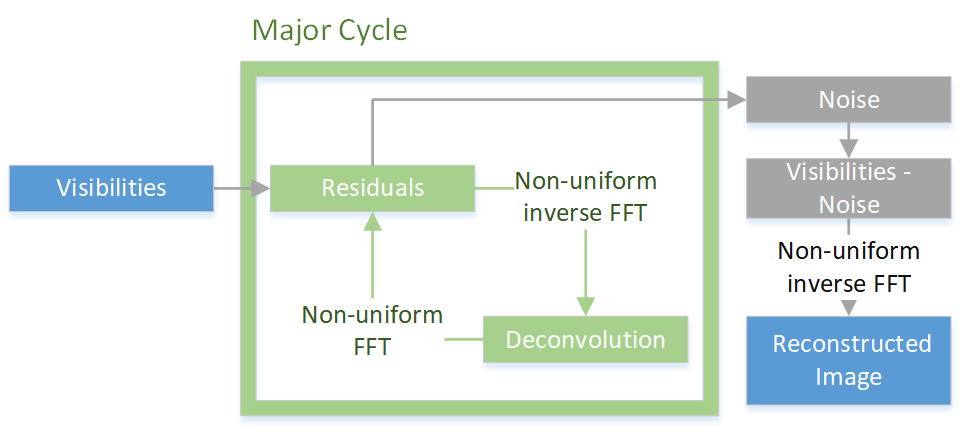
\includegraphics[width=0.80\linewidth]{./chapters/01.intro/Major-Minor.png}
	\caption{The Major Cycle Framework}
	\label{intro:major}
\end{figure}

The CLEAN objective \eqref{intro:clean} assumes that the observed image has few non-zero pixels, i.e. is sparse in the image domain. When the interferometer observed an image with only stars, which are concentrated on a single pixel, the observed image is at the minimum of the CLEAN objective. 

Current Compressed Sensing reconstructions also use the non-uniform FFT and cycle between Visibility and image space\cite{girard2015sparse,dabbech2018cygnus}. Although they do not use a deconvolution on the image, one can make the argument that they do not use the Major Cycle architecture. One of the main reasons why Compressed Sensing reconstructions are more expensive is because they need more non-uniform FFT cycles. Current research is focused on reducing the number of cycles\cite{dabbech2018cygnus}. However, since the non-uniform FFT is central to the Major Cycle, many approximations for realistic Interferometers made in section \ref{meerkat} can be used by the Compressed Sensing approaches. They are functionally similar. In this work, we group CLEAN and Compressed Sensing reconstructions with the non-uniform FFT together in the Major Cycle architecture.

 






